\section{Reproduction of ICL of linear functions}
% (b) your reproduction, with a short log of what the paper left unspecified and what you had to guess

\subsection{Setup}
We train our own transformer from scratch on an NVIDIA A100 via Modal, using the same
model, optimiser, curriculum and
number of training steps as \cite{garg2022what}. As in the paper, we evaluate on 1280
prompts with 90\% bootstrap confidence intervals.

The paper does not state how many training runs its main results are based on, and the
authors released one checkpoint per task. We train a single run. Since neither their code
nor ours fixes a random seed, our error bars reflect variation over evaluation prompts
only. Otherwise we differ only in software (Python 3.10 instead of 3.8) and hardware
(A100 instead of RTX 3090), which change neither the model nor the training procedure.

\subsection{Results}

\paragraph{Clean labels.}
The transformer outperforms 3-NN and averaging, and its error closely tracks that of
minimum-norm least squares (Figure~\ref{fig:linear}, Table~\ref{tab:linear-repro}),
including the drop to zero error at $k \geq 20$, where the 20-dimensional problem is
fully determined and least squares has a unique solution.

\paragraph{Noisy labels.}
With noisy labels, the transformer still outperforms 3-NN and averaging, and reproduces
the double descent curve (Figure~\ref{fig:noisy}). For minimum-norm least squares, this
curve appears when test error is plotted against the number of noisy training samples
$n$ for a fixed number of features $p$ (here $n = k$, $p = d = 20$). For $n < p$, the
system is underdetermined. Among the infinitely many exact fits, the minimum-norm
solution keeps the weights small and spreads the noise over many directions, so
predictions on new data stay reasonable. At $n = p$, the fit is unique and must pass
through every noisy label. This requires large weights, which turn label noise into large
test errors, so the error peaks. For $n > p$, the problem is overdetermined and the noise
averages out as $n$ grows. Interestingly, the transformer handles the peak at $n = p$
better than minimum-norm least squares. This possibly suggests some kind of
regularisation of the in-context learned weights that keeps them from taking extreme
values.

\paragraph{Comparison with the released checkpoints.}
Our transformer performs like the checkpoints released by \cite{garg2022what}, up to
random variation; see Appendix~\ref{app:reproduction}.

\begin{figure}[H]
\centering
\begin{subfigure}[t]{0.38\textwidth}
  \centering
  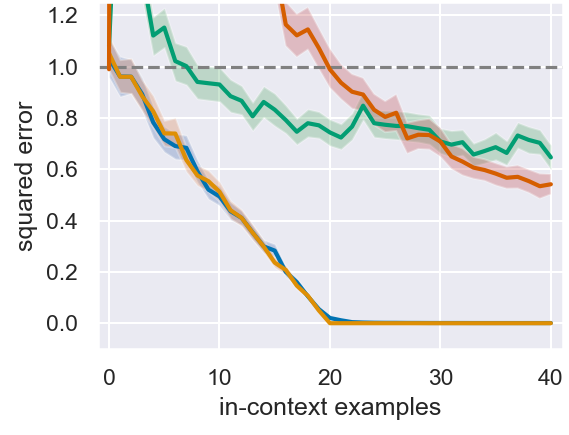
\includegraphics[width=\linewidth]{figures/standard_repr_cropped.png}
  \caption{Clean labels}
  \label{fig:linear}
\end{subfigure}\hfill
\begin{subfigure}[t]{0.58\textwidth}
  \centering
  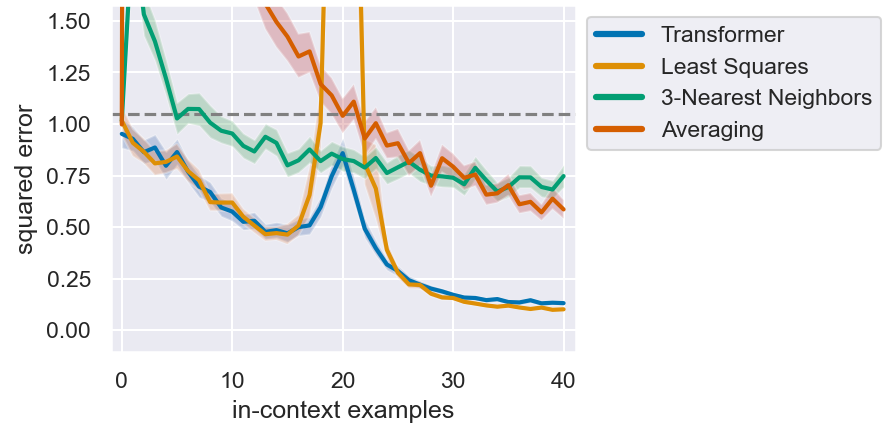
\includegraphics[width=\linewidth]{figures/noisyLR_repr_cropped.png}
  \caption{Noisy labels}
  \label{fig:noisy}
\end{subfigure}
\caption{ICL performance of our trained transformer on linear functions.}
\label{fig:repr}
\end{figure}